\section{Profondità ottica}\label{sec:profondità-ottica}
Per realizzare un modello dell'atmosfera stellare si procede in maniera simile alla modellizzazione dell'interno stellare. Tuttavia, come variabile, invece della distanza dal centro, $r$, si utilizza la \emph{profondità ottica}. Infatti, le distanze dal centro sono molto elevate, pertanto è conveniente avere una misura della distanza dalla superficie della stella. 

\subsection{Profondità ottica verticale}
La profondità ottica è definita nella seguente maniera:
\begin{equation}\label{eq:profondità-ottica-atmosfera}
    \tau_\lambda = \int \kappa_\lambda \rho \ud S
\end{equation}
dove $\kappa$ è l'opacità, misurata in $\si{cm^2.g^{-1}}$, $\rho$ è la densità di massa, misurata in $\si{g.cm^{-3}}$ e $S$ rappresenta la distanza lungo una direzione radiale, misurata in $\si{cm}$.



In particolare, $\tau_\lambda = 0$ sulla superficie della stella, mentre $\tau_\lambda$ cresce andando verso il centro, seguendo un cammino radiale. Come si può notare in fig.~\ref{fig:profondita-ottica-atmosfera}, la profondità ottica \emph{non} è una misura \emph{unica} della distanza dalla superficie, infatti, se considero raggi con direzioni diverse, ottengo profondità ottiche diverse. Per utilizzare questa grandezza per misurare univocamente le distanze, si considera la \emph{profondità ottica verticale}, dove integro lungo una direzione radiale:
\begin{equation}\label{eq:profondità-ottica-verticale}
    \tau_{\lambda, V} = \int_z^0 \kappa_\lambda \rho \ud z
\end{equation}
dove la direzione identificata da $z$ è perpendicolare alla superficie della stella. A questo punto possiamo utilizzare la profondità ottica per determinare quale è lo strato più interno dal quale la radiazione a una data lunghezza d'onda riesce ad emergere verso l’esterno, o, in altre parole, la profondità ottica mi dice quanto è schermata la radiazione che viene dall'interno. D'ora in poi, quando si parlerà di profondità ottica si farà riferimento alla profondità ottica verticale.

\begin{figure}
    \centering
    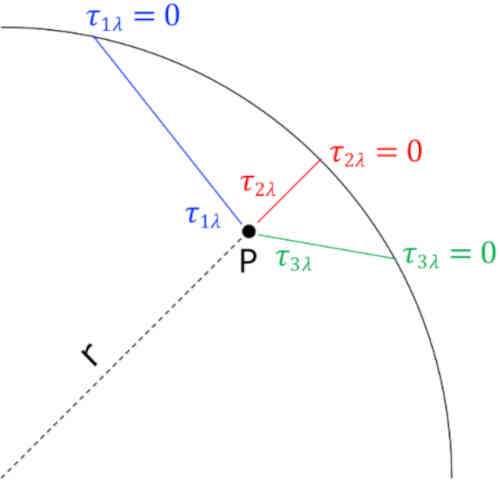
\includegraphics[width=0.3\textwidth]{immagini/profondita-ottica-atmosfera.jpg}
    \caption{La profondità ottica non è una misura univoca della distanza dalla superficie. Se scelgo tre direzioni radiali, in blu, rosso e verde, ottengo prodondità ottiche diverse in uno stesso punto P, in particolare $\tau_{1\lambda} \neq \tau_{2\lambda} \neq \tau_{3\lambda}$. L'unica cosa uguale per le tre situazioni è che in superficie la profondità ottica è nulla.}
    \label{fig:profondita-ottica-atmosfera}
\end{figure}

\subsection{Temperatura effettiva}
Sia la profondità ottica che la temperatura aumentano andando verso il centro della struttura stellare. La loro relazione definisce univocamente la così detta \emph{temperatura effettiva} della stella, ed è un'equazione chiave per un modello di atmosfera:
\begin{equation}\label{temperatura-effettiva}
    T^4 = \frac{3}{4} {T_e}^4 \bigl( \tau_\nu + \frac{2}{3} \bigr)
\end{equation}
La temperatura effettiva $T_e$ è la temperatura alla quale la profondità ottica vale $\tau_\lambda = 2 / 3$. Posso interpretare lo strato in cui ciò è vero come lo strato più interno da cui riesce ad emergere la radiazione. Per il sole, ad esempio, si ha $T_e = \SI{5770}{K}$.

